\documentclass{article}
\usepackage{graphicx}
\begin{document}	
{\begin{center}
		
	\end{center}\Huge\textbf{Piyush Agarwal}}
\\
\rule{\paperwidth}{0.2ex}
C-6 Ganga Apartment,\hspace{24ex} Contact: 9730816000
\\
Hilltop Layout, \hspace{32ex} e-mailid: piyushagarwal190@gmail.com
\\
Nagpur- 440010 
\\
Maharashtra
\begin{flushright}
	\begin{figure}[h]
		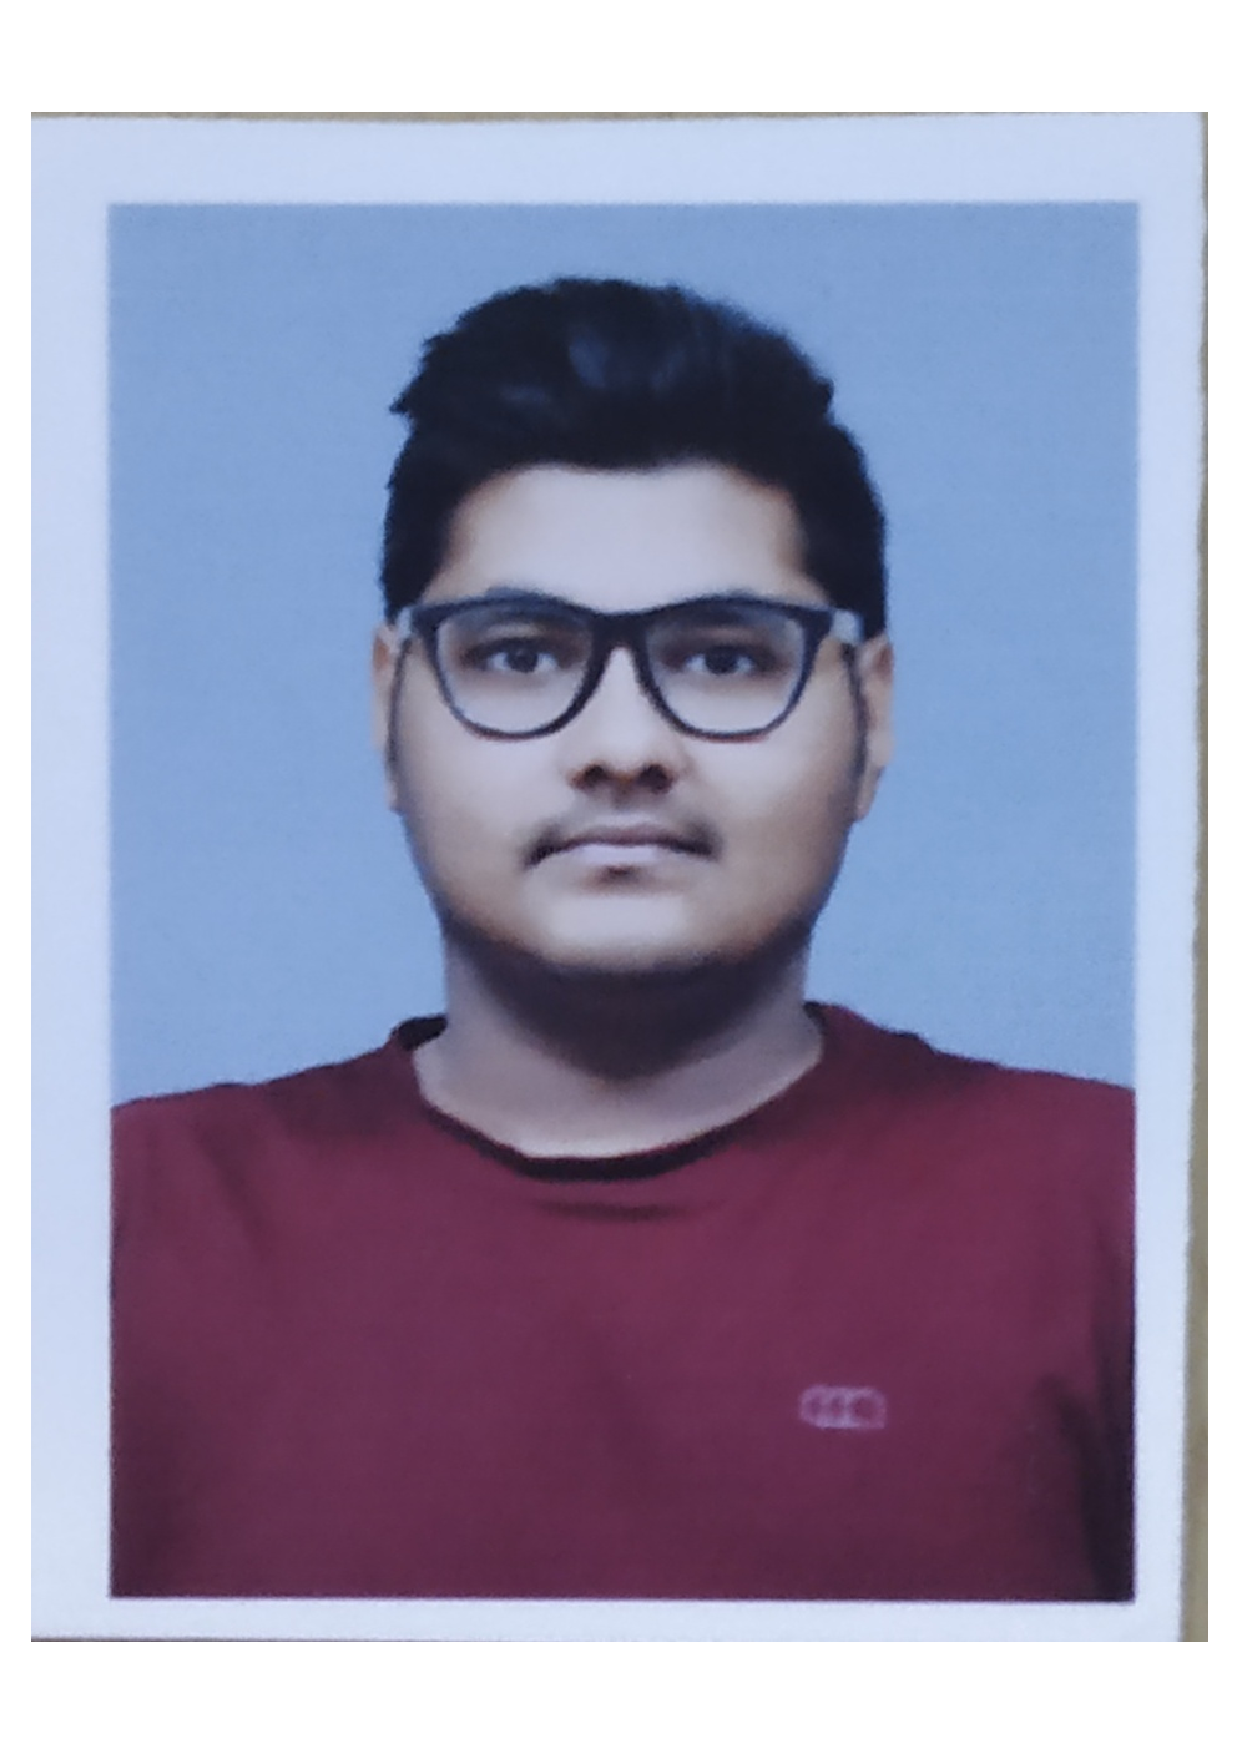
\includegraphics[width=15ex]{PIYUSH7}
	\end{figure}
\end{flushright}
\section{Objective}
{\large To develop my knowledge and to enhance my personal growth and to gain practical experience.}
\section{Education}
\begin{tabular}{ |p{3cm}|p{3cm}|p{3cm}|p{2cm}|p{3cm}| }
	\hline
	Degree& College/School &University/Board &Passing Year &Pass Percentage 
	\\
	\hline
	\hline
	SSC & St.Xaviers's High School &CBSE &2014 &91 \\
	\hline
	HSC & Gondia Public School   & CBSE &2016 &85 \\
	\hline
	B.tech &Shri Ramdeobaba College of Engineering and Management & RTMNU &2020 &Pursuing \\
	\hline
\end{tabular}
\section{Training and Internship}
\begin{itemize}
	\item{ Somebuddy Pvt.ltd
		\begin{itemize}
			\item Wordpress and Seo Intern
	\end{itemize}}
	\item { Internshala
		\begin{itemize}
			\item Digital Marketing Training
	\end{itemize}}
\end{itemize}
\section{Mini Projects}
\begin{enumerate}
	\item Random Number Generator using 8051
	\item Gas Leakage using LPG module
	\item Voltage Multiplier
\end{enumerate}
\section{Technical Skills}
\begin{itemize}
	\item Basics of C,C++
	\item Wordpress
	\item Google-Analytics
	\item Digital Marketing
\end{itemize}
\section{Soft Skills}
\begin{enumerate}
	\item Adaptibilty
	\item Synergy
	\item Positive thinking
	\item Handling Pressure
\end{enumerate}
\section{Extra Curricular Activities}
\begin{itemize}
	\item{ Committees
		\begin{itemize}
			\item Entrepreneurship and Development
			\item Rotaract Club
			\item Literary Team
			\item TBI cell
	\end{itemize}}
	\item { Participations
		\begin{itemize}
			\item Transpreneur
			\item StartupFest at IYC
			\item CEO event at VNIT
	\end{itemize}}
\end{itemize}
\section{Co-Curricualar Activities}
\begin{enumerate}
	\item E-yantra Robotics Competetion
	\item Techfest at IIT-B
	\item AXIS at VNIT
\end{enumerate}
\section{Personal Details}
Father's name: Mr.Pawan Agarwal \\
Mother'sname: Ms.Seema Agarwal \\
Sex: Male \\
Date of Birth: 10th April 1998\\
Nationalty: Indian\\
Marital Status: Unmarried\\
\section{Reference}
\begin{enumerate}
	\item Google
	\item Teacher
\end{enumerate}
\section{Declaration}
I solemnly declare that all the above information is correct to the best of my knowledge and belief.
\end{document}

